% Chapter Template

\chapter{Implementation} % Main chapter title

\label{Chapter7} % Change X to a consecutive number; for referencing this chapter elsewhere, use \ref{ChapterX}

\lhead{Chapter 8. \emph{Implementation}} % Change X to a consecutive number; this is for the header on each page - perhaps a shortened title

%----------------------------------------------------------------------------------------
%	SECTION 1
%----------------------------------------------------------------------------------------

\section{Overview}

This chapter deals with practical programming issues and conceptual perspectives on the implementation of the CCDT-1 equation for the system described in chapter \ref{Chapter6}.

As was clear from the derivation of the equations in chapter \ref{Chapter5}, the CCDT-1 consists of a CCD with an addition just 4 diagrams from the CCDT $t2$ and $t3$ equation. A natural stepping stone in the implementation is therefore the CCD equations, as they will also serve as means of benchmarking and validating the solver against existing results. 

No CCM results beyond the CCD (with CCD(T) performed by Shepherd and Gruneis \cite{Shepherd2013c}) is known to the author at the time of this thesis, so direct benchmarking and validation of the CCDT-1 to prior calculations is not possible. To mend this shortcoming, we will develop two independent solvers for the CCDT-1 so that some corroboration of the results is possible. This approach will also be of great aid in the debugging process, as it will allow for extensive comparison and testing of subprocesses.

We will refer to the two solvers as the \emph{block} implementation and the \emph{sparse} implementation, and the reason for the naming will become clear in the upcoming discussion. While both solvers have similar aims, they are founded on two conceptually different perspectives on the equations involved. 

The sparse implementation approaches the problem in such a way the code very closely resembles the actual equations. One advantage of this is that it to an extent ensures the validity of the results, although bugs and misinterpretations are bound to occur. While memory usage of this approach is optimal, it has turned out that the actual iterative steps performs sub optimal.

The block implementation is built for the purpose of highly efficient computations and minimal memory usage. It is much more abstract in its comparison with the actual equations than the sparse solver, and it is to a large extent based on physical symmetries and restrictions present in the system. 

Our strategy in this thesis is therefore to implement both solvers, whereby we validate both against the CCD results present in the literature (see Refs.~\cite{Baardsen2014, Roggero2013, Shepherd2012a, Shepherd2012, Shepherd2013, Shepherd2013c}). We then corroborate the CCDT-1 results by ensuring consistency between the solvers. We are then finally able to perform the calculations presented in the final chapter of this thesis.


\subsection{The problem}

While a lot of computational \emph{results} are present in the literature, the author has not been able to find any descriptions of the actual algorithms used. In the literature, we find that corresponding CCD calculations for the HEG normally extrapolates results from basis sets of up to around 2000 particle states \cite{Shepherd2014, Roggero2013}, while some may even go as high as 20000 particle states \cite{Baardsen2014}. 

Most descriptions of the actual algorithms for the coupled cluster method very closely resemble the code generated from CCAlgebra (see Ref.~\cite{CCAlgebra}) as presented in chapter \ref{Chapter5}. Such implementations may be called \emph{naive}, as they have a one to one correspondence with the equations; each sum is translated into a nested for-loop, each diagram is added term by term, and at the bottom of each cluster of nested for-loops lies a couple of function calls and a multiplication. In the same way, we may refer to the storage of amplitudes and interactions as \emph{naive}, if it has a one to one correspondence with the tensor representation in the equations. This would mean that we also store all elements equal to zero, neglecting any sparsity in the system.

Even with the inclusion of intermediates, such a naive approach to our system would be futile. The $t3$ amplitude is a tensor of rank 6, and if we were to naively store it for 14 particles using arrays it would scale roughly as shown in Fig. \ref{fig:naive_t3}. This results in some serious limitations to the size of the basis, so we clearly need to move beyond any naive storage implementation.

Since the interaction that occurs in this system is defined by a product of Kronecker deltas over quantum numbers, we may expect most of the terms that occur in the diagrams to be zero. This fact actually reflects the conservation of momentum and spin in the system. The excitations due to the cluster operator should conserve spin and total momentum for the system. This is a strong indication that our system will be very sparse, and that alternative data structures to the naive one should be explored.

\begin{figure}[p]
    \centering
    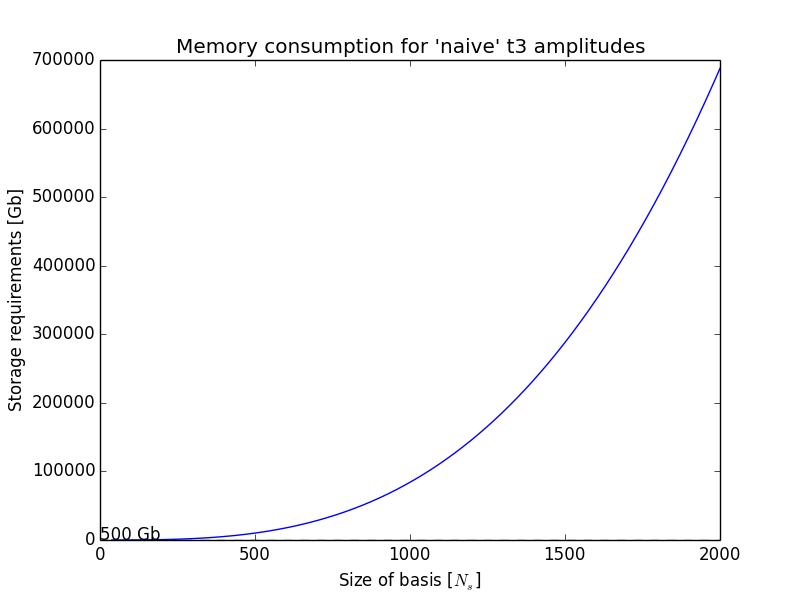
\includegraphics[width=0.8\textwidth]{naive_t3}
    \caption{Size of the $t3$ amplitudes as a function of the number of particle states for a naive implementation, where the sparsity of the system is ignored.}
    \label{fig:naive_t3}
\end{figure}

To investigate the physical system properly with this method we will therefore need to write our code in a way that limits the use of memory and at the same time achieves optimal performance. 


\section{Contractions as matrix multiplications}

We will need to generate diagrams, which are contractions between tensors of varying rank (at most 6). Common to both implementational approaches is that we shall conceptually consider diagrams as matrix multiplications. Bluntly speaking, and probably not in full accordance with linear algebra formalism, matrix multiplication  \emph{is already} a special case of contraction between two or more tensors of rank 2. Consider for example the matrix-matrix product

\begin{equation}
(MN)^\alpha_\gamma = \sum_\beta M^\alpha_\beta N^\beta_\gamma .
\end{equation}

If we allow ourselves a more liberal approach, we may as well define

\begin{equation}
(MN)^\alpha_\gamma = \sum_\beta M^\beta_\alpha N^\beta_\gamma \rightarrow  M^T N.
\end{equation}

In \ref{Chapter5}, we interpreted contractions as sums over internal lines in the diagrams. The same may be done for the matrix multiplication above. We still need to define tensors of rank $\geq 2$ as matrices for this to make full sense.

The motivation for introducing this concept, is twofold. Firstly it will - perhaps surprisingly - give a significant speedup of the solvers, while secondly it provides a suitable simplification of the actual coding process. A lot of nested for loops over varying indices may be subject to a number of mis-spellings/labelings or other kind of errors.  

For optimal performance, we need to utilize BLAS (Basic Linear Algebra Subprograms) (see Ref.~\cite{BLASsite}) where possible. BLAS has three levels of operation depending on the order of the computational complexity. The optimization of operations is achieved by carefully utilizing the Level 1 and Level 2 cache, to reduce the cost assosciated with memory access \cite{Karniadakis}. The most efficient level of operation is BLAS Level 3, or operations of $\mathcal{O} (n^3)$, such as matrix-matrix multiplication \cite{Karniadakis}

To most efficiently perform all the floating point operations involved in this implementation, we therefore want to perform contractions as matrix-matrix multiplications. This basically means that we need to set up matrices for the interaction and the amplitudes, and align the elements in these matrices so that each resulting element contains the same sums as defined in the diagram.

\subsection{Mapping diagrams onto matrices}

In the same way that a Picasso painting preserves details beyond the line of sight, we will need to unambiguously map tensors of rank $\geq 2$ onto matrices in such a ways that all elements are present and consistent amongst the matrices. One possibility for the interaction and the $t2$ amplitude, is

\begin{equation}
\langle p q \vert \hat{v}\vert r s \rangle = V_{\alpha(p,q), \beta(r,s)}.
\label{eqn:t2mapping}
\end{equation}

Where 

\begin{equation}
\alpha(p,q) = p + qN_p, \hspace{1cm}
\beta(r,s) = r + sN_r.
\label{eqn:t2mapping2}
\end{equation}

Note that the "steplength" of the second index equals the number of unique states in front of it. 

The above is easily extended to the $t3$ amplitude:

\begin{equation}
t^{abc}_{ijk} = t_{\alpha(a,b,c), \beta(i,j,k)},
\label{eqn:t3mapping}
\end{equation}

where 

\begin{equation}
\alpha(a,b,c) = a + bN_a + cN_aN_b,
\hspace{1cm}
\beta(i,j,k) = i + j*N_i + k*N_i*N_j.
\label{eqn:t3mapping2}
\end{equation}

The corresponding index $\alpha,\beta$ will now correspond to the row and column in the matrices, respectively. 

\subsection{Subdividing the interaction matrix}


\begin{figure}[p]
    \centering
    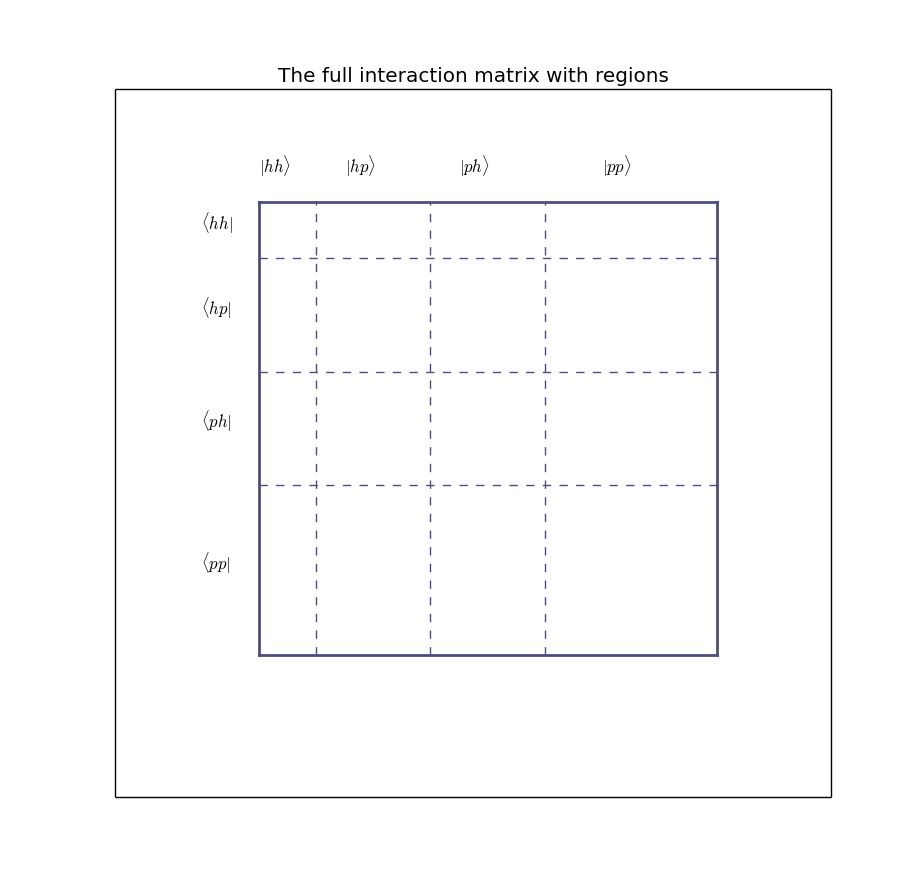
\includegraphics[width=0.8\textwidth]{interaction_matrix}
    \caption{The interaction matrix with regions. The subdivision into regions is made so that each submatrix may be loaded when calculating the different diagrams. The difference in size is meant to illustrate that we will normally consider more particle states than hole states.}
    \label{fig:interaction_matrix}
\end{figure}


Diagrams naturally include terms summing over particle- or hole states. In no cases do we sum over \emph{all} the states (particles and holes) so we generally find matrix elements of the form $\langle pp \vert \vert pp \rangle $, $\langle pp \vert \vert hh \rangle $, $\langle hp \vert \vert ph \rangle $ and so on.  There is a lot of symmetries that occur in the interaction matrix, so it will make sense to divide it into smaller regions. We will refer to these regions by their configuration in terms of particle- and hole states, as this is the way they occur in the diagrams. This subdivison is illustrated in \ref{fig:interaction_matrix}. For example, when we consider diagrams where the interaction has the form $\langle i j \vert \vert a b\rangle$, we will refer to the submatrix as the hh-pp matrix (hole-hole, particle-particle).

The off-diagonal submatrices in the interaction matrix have their transposed counterparts mirrored across the diagonal, and of course the usual symmetries due to the nature of spin in the two body interaction in Eq. (\ref{eqn:twobody}) apply shown in table \ref{tab:symmetries_t2}. 



\begin{table}[]
\centering
\caption{Spin symmetries in the two body interaction matrix}
\label{tab:symmetries_t2}
\begin{tabular}{lllll}
$\langle \Up{p} \Up{q} \vert \vert  \Up{r} \Up{s} \rangle $ & $=$ & $\langle pq \vert \hat{v} \vert rs \rangle - \langle pq \vert \hat{v} \vert sr \rangle$ \\  
$\langle \Dn{p} \Dn{q} \vert \vert  \Dn{r} \Dn{s} \rangle $ & $=$ & $\langle pq \vert \hat{v} \vert rs \rangle - \langle pq \vert \hat{v} \vert sr \rangle$ \\  
$\langle \Up{p} \Dn{q} \vert \vert  \Up{r} \Dn{s} \rangle $ & $=$ & $\langle pq \vert \hat{v} \vert rs \rangle$ \\  
$\langle \Dn{p} \Up{q} \vert \vert  \Dn{r} \Up{s} \rangle $ & $=$ & $\langle pq \vert \hat{v} \vert rs \rangle$ \\  
$\langle \Dn{p} \Up{q} \vert \vert  \Up{r} \Dn{s} \rangle $ & $=$ & $-\langle pq \vert \hat{v} \vert rs \rangle$ \\  
$\langle \Up{p} \Dn{q} \vert \vert  \Dn{r} \Up{s} \rangle $ & $=$ & $-\langle pq \vert \hat{v} \vert rs \rangle$ \\  
$\langle \Up{p} \Up{q} \vert \vert  \Dn{r} \Dn{s} \rangle $ & $=$ & $0$ \\  
$\langle \Up{p} \Up{q} \vert \vert  \Dn{r} \Up{s} \rangle $ & $=$ & $0$ \\  
$\langle \Up{p} \Up{q} \vert \vert  \Up{r} \Dn{s} \rangle $ & $=$ & $0$ \\  
$\langle \Dn{p} \Dn{q} \vert \vert  \Up{r} \Up{s} \rangle $ & $=$ & $0$ \\  
$\langle \Dn{p} \Dn{q} \vert \vert  \Dn{r} \Up{s} \rangle $ & $=$ & $0$ \\  
$\langle \Dn{p} \Dn{q} \vert \vert  \Up{r} \Dn{s} \rangle $ & $=$ & $0$ \\  
$\langle \Dn{p} \Up{q} \vert \vert  \Up{r} \Up{s} \rangle $ & $=$ & $0$ \\  
$\langle \Up{p} \Dn{q} \vert \vert  \Up{r} \Up{s} \rangle $ & $=$ & $0$ \\  
$\langle \Up{p} \Dn{q} \vert \vert  \Dn{r} \Dn{s} \rangle $ & $=$ & $0$ \\  
$\langle \Dn{p} \Up{q} \vert \vert  \Dn{r} \Dn{s} \rangle $ & $=$ & $0$ \\  
\end{tabular}
\end{table}


\subsection{Aligning matrices}

In lack of a better word, we shall refer to the different ways in which higher dimensional tensors are mapped onto matrices as their \emph{alignment}. Each element in the tensor will need to be assigned an index in the matrix, and these should be chosen such that the resulting matrix-matrix multiplications corresponds to the contractions specified in the diagrams.

Some diagrams align perfectly in the row and columns "out of the box". Consider for example the $L_a$ "ladder" term \cite{ShavittBartlett2009} (see table \ref{tab:CCD_diagrams1}), where

\begin{equation}
L_a = \sum_{cd} \langle a b \vert \hat{v}\vert c d \rangle t^{cd}_{ij}.
\label{eqn:L1diag}
\end{equation}

Here, we see that the columns in the interaction matrix aligns, since the mapping in Eqn. (\ref{eqn:t2mapping}) will result in 

\begin{equation}
 \langle a b \vert \hat{v}\vert c d \rangle \equiv v^{ab}_{cd}  \rightarrow v^{\alpha(a,b)}_{\beta(c,d)},
\end{equation}

\begin{equation}
t^{cd}_{ij}  \rightarrow t^{\beta(c,d)}_{\gamma(i,j)}.
\end{equation}

Now by definition, obviously 

\begin{equation}
\beta(c,d) = \beta(c,d),
\end{equation}

so that

\begin{equation}
(L_a)^{\alpha}_{\gamma} = \sum_{\beta} v^\alpha_\beta t^\beta_\gamma \rightarrow L_a = v t.
\label{eqn:L1diag_mapped}
\end{equation}

In other cases we are not that lucky. We may for example consider the $L_c$ term, where

\begin{equation}
L_c  = -P(ba)P(ij)  \sum_{ck} \langle ak \vert \vert cj \rangle t_{ik}^{cb}.
\end{equation}

Just naively mapping onto the matrices will result in

\begin{equation}
 \langle ak \vert \hat{v}\vert cj \rangle \equiv v^{ak}_{cj}  \rightarrow v^{\alpha(a,k)}_{\beta(c,j)},
\end{equation}

\begin{equation}
t^{ik}_{cb}  \rightarrow t^{\beta(i,k)}_{\gamma(c,b)}.
\end{equation}

The matrix multiplication is "misaligned":

\begin{equation}
L_c  \neq -P(ba)P(ij) v^{\alpha(a,k)}_{\beta(c,j)} t^{\beta(i,k)}_{\gamma(c,b)}.
\end{equation}

This will not work, and doesn't even provide us with compatible matrix sizes that allow for such a multiplication to be performed. What we instead want, is to find a mapping so that

\begin{equation}
 v^{ak}_{cj}  \rightarrow \tilde{v}^{\alpha(a,j)}_{\beta(c,k)},
\end{equation}

\begin{equation}
t^{ik}_{cb}  \rightarrow  \tilde{t}^{\alpha(c,k)}_{\beta(b,i)}.
\end{equation}

This will allow us to calculate

\begin{equation}
\tilde{L_c}  = -P(ba)P(ij) \tilde{v}^{\alpha(a,j)}_{\beta(c,k)} \tilde{t}^{\alpha(c,k)}_{\beta(b,i)}.
\end{equation}

This will provide us with an "unaligned" $L_c$ denoted $\tilde{L_c}$ that may be "realigned" so it fits into the diagram summation in the $t2$ amplitude:

\begin{equation}
\tilde{(L_c)}^{\alpha(a,j)}_{\beta(b,i)} \rightarrow {(L_c)}^{ab}_{ij}.
\end{equation}

We will also have situations where contractions occur in more or less than two indices, so that our mapping cannot be directly applied. In these situations we introduce a general mapping rule, which states that a mapped index of elements $n_a .. n_N$ in the order given by their numeric subindices and with the number of elements in each place $N_a, N_b ... N_N$ may be expressed as

\begin{equation}
\alpha(a,b,c,...,N) \equiv abc..N = n_a + n_bN_a + n_cN_aN_b + n_dN_aN_bN_c + ... + n_N \prod_i^{N-1} N_i  .
\end{equation}

As long as this rule is consistently applied to each mapping of multiple particle or hole states onto rows or columns of the matrix, it will allow us to perform contractions over any number of states as matrix-matrix multiplications. 

To demonstrate this, we consider finally the $D_{3d}$ diagram \ref{tab:CCD_diagrams1}, where 

\begin{equation}
D_{3d}= -\frac{1}{2} P(ij) \sum_{cdkl} \langle kl \vert \vert cd \rangle t_{ik}^{cd} t_{jl}^{ab}.
\end{equation}

Here we have both a quadratic contribution from the $t2$ amplitudes and contractions of three lines between the interaction and the first, and only one contraction between the interaction and the last. We need to align the following matrices

\begin{equation}
v^{kl}_{cd} \rightarrow \tilde{v}_{kcd}^{l},
\end{equation}

\begin{equation}
t_{ik}^{cd} \rightarrow \tilde{t}^{kcd}_i,
\label{eqn:align_t2}
\end{equation}

\begin{equation}
t_{jl}^{ab} \rightarrow \tilde{t}^{jab}_l,
\end{equation}

so we may compute the unaligned diagram

\begin{equation}
(\tilde{D}_{3d})^{jab}_{i} = \tilde{t}^{jab}_l \tilde{v}_{kcd}^{l}  \tilde{t}^{kcd}_i,
\end{equation}

and then realign the diagram so it will be possible to sum it into the equation

\begin{equation}
 (\tilde{D}_{3d})^{jab}_{i} \rightarrow (D_{3d})^{ab}_{ij}.
\end{equation}

\subsection{Use of non standard terminology}

By referring to this processes of \emph{alignment} we have probably introduced some non standard terminology. There may exist corresponding and better expressions in use, but the author has not been able to find them in the literature due to the lack of implementational descriptions. From a theoretical point of view, it may be argued that the process of alignment is just a generalization of matrix transposition for tensors of any rank.We shall however use this terminology throughout this thesis with the reservation that better expressions may exists.



\section{The sparse matrix approach}

We have already mentioned the sparsity of our system, and we have explored how interactions and amplitudes may be represented by matrices. It is then only natural to consider whether a sparse matrix-matrix  multiplicaton scheme may be beneficial and efficient for the system. At least, as we shall see, it is in principle simple to implement such a scheme and extend it to any order of the CC equations.

A matrix is generally considered sparse if most of its elements are zero \cite[p.122]{Lay}. As a rough estimate of the sparsity of our system, we may consider all interactions between particle states for a given number of basis states. These interactions is involved in the calculation of the $L_a$ ladder term in the CCD approximation  \cite{ShavittBartlett2009}, and it is the most time consuming diagram in the calculation due to the number of states involved. By defining the density as the fraction of terms in the $L_a$ sum that is nonzero, we see from Fig. \ref{fig:density_vpppp} that the density seems to converge to somewhere below 0.01 percent as the number of particle states increases.

In such systems as ours, we will benefit from the implementation of a sparse matrix-matrix multiplication solver given that the arrangement of the elements in the matrix is completely random. As we shall see when considering the block implementation, this last part is not the case in our system. 

\begin{figure}[p]
   \centering
   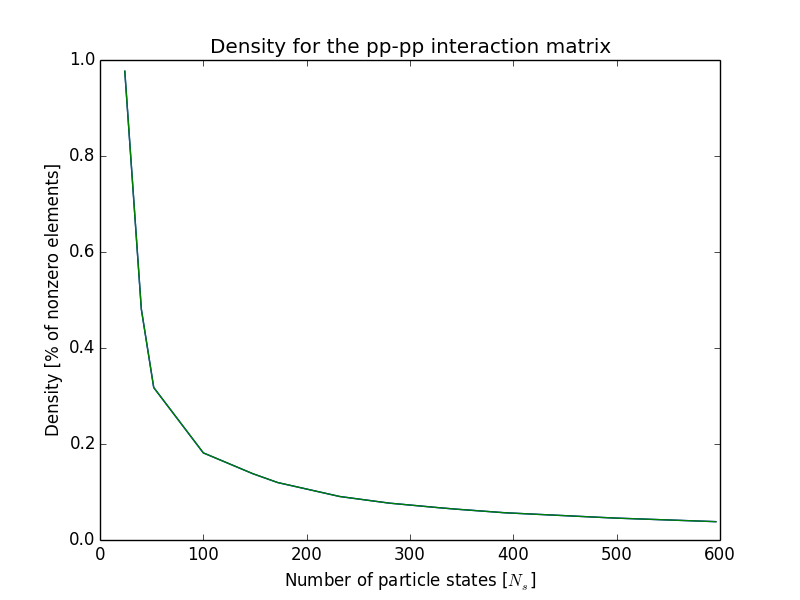
\includegraphics[width=0.8\textwidth]{density_pppp}
   \caption{Density of the $\langle pp \vert \vert pp \rangle$ interaction matrix. The density seems to converge towards somewhere below $0.1$ percent, providing a reasonable argument for the use of sparse matrices.}
   \label{fig:density_vpppp}
\end{figure}

\FloatBarrier

\section{Sparse matrix storage}

Sparse matrices are a commonly used data structure in computations where matrix elements are mostly zero. There exists a number of different formats, such as the COOrdinate format, CRS and CCS \cite{sparseformats}, with well defined and efficient algorithms for matrix-vector or matrix-matrix multiplication. 

The general idea is to store only three arrays; one containing the actual elements, and two others containing their corresponding indices in the full matrix. This is basically the COO format shown in table \ref{tab:coo_storage} with its dense interpretation in table \ref{tab:coo_storageII}. By sorting and compressing either the row or column arrays, one get the CRS or CCS formats respectively. These both reduce the spaces needed for storage somewhat, but also sorts the elements in such a way that matrix-matrix multiplications may be performed more efficiently. The backside is the fact that the sorting procedure may be relatively costly for large arrays.

\begin{table}[]
\centering
\caption{Sparse matrix storage (COOrdinate format)}
\label{tab:coo_storage}
\begin{tabular}{llllllll}
Elements & a & b & c & d & e & f \\ \hline
row          & 1 & 1 & 2 & 3 & 5 & 5 \\ \hline 
column    & 0 & 3 & 1 & 2 & 1 & 3 \\ \hline
\end{tabular}
\end{table}

\begin{table}[]
\centering
\caption{Sparse matrix storage (COOrdinate format) as dense matrix}
\label{tab:coo_storageII}
\begin{tabular}{llllllll}
0 & 0&0 &0 &  \\
a&0 &0 &0 &  \\
0 &c&0 &0 &  \\
b&0 &d&0 & \\
0 &0  & 0 &0 & \\
0 &e& 0 &f& \\
\end{tabular}
\end{table}

\section{Sparse tensor storage}

Matrices are tensors of rank $=2$. Generalizing the ideas used in the COO format, we may define a sparse tensor storage that works for tensors of any rank. This does really not involve anything else than having an optional number of element index arrays (rows and columns) available for the sparse tensor. For example, we may store the $t^{ab}_{ij}$ tensor as in table \ref{tab:flexmat_class}.

\section{Sparse matrix alignment}

When considering how these sparse tensor elements are stored in conjunction with the alignment principles discussed previously, it is clear that the process of aligning sparse tensors will become remarkably simple. For example, we may perform the process in equation \ref{eqn:align_t2} simply by calculating

\begin{equation}
rows = k + cN_k + dN_kN_c = k + cN_h + dN_hN_p,
\end{equation}

and

\begin{equation}
cols = i.
\end{equation}

And then initialize a sparse matrix with the elements in the same order as they appear in the sparse tensor data structure, but with columns and rows as produced by the alignment process. 


\begin{table}[]
\centering
\caption{Sparse tensor storage (COOrdinate format)}
\label{tab:flexmat_class}
\begin{tabular}{llllllll}
Elements & $e_0$ & $e_1$ & $e_2$ & $e_3$ & $e_4$ & $e_5$ \\ \hline
c          & 1 & 1 & 2 & 3 & 5 & 5 \\ \hline 
d    & 0 & 3 & 1 & 2 & 1 & 3 \\ \hline
i   & 6 & 7 & 7 & 3 & 13 & 13 \\ \hline
k    & 11 & 3 & 1& 1 & 4 & 6 \\ \hline
\end{tabular}
\end{table}



\FloatBarrier

\section{The sparse matrix implementation}

The sparse matrix approach was implemented both in python and C++, but we will here only focus on the C++ implementation. To handle linear algebra operations, for vectors, matrices and sparse matrices, the linear algebra library Armadillo was extensively used (see Ref.~\cite{Armadillo}). Armadlillo also utilize all levels of BLAS, so it ensures optimal performance given a well written implementation. The implementation has no other dependencies aside from OpenMp and Armadillo. 

The implementation is made in an object oriented manner, utilizing multiple classes for solvers, basis initialization, and tensor initialization. We will briefly discuss each class and how they fit in with the full picture.

\subsection{Amplitude storage}

Two different classes were implemented to store and align the $t2$ and $t3$ amplitudes, namely the \emph{flexmat} and \emph{flexmat6} classes respectively. The number 6 refers to the rank of the tensor. 

These classes utilize the COO storage as specified for tensors of rank $\geq 2$ (see table \ref{tab:flexmat_class}), and allows for relatively efficient alignment of elements in the different diagrams. The inverse process of realigning incoming unaligned diagrams is also possible. 

Although it is good coding practice to avoid repeating oneself (see Ref.~ \cite{DRY}), a great deal of the functionality of this code was autogenerated with a python script, resulting in a lot of similar functions. The motivation for this approach is twofold; it allows for a syntax that is very easily understood in terms of the different diagrams that occur in the CC equations, which allows the actual implementation of the equations to be written very compactly and easily interpreted by humans. Secondly, this is an easy way to write highly specialized code for generating all possible alignments of elements needed for an implementation where this is not known in advance. One could also argue that this is not the same as repeating oneself, as the actual code is easily changed by small changes in the script generating the code. 

An alternative to this could be to write one single function that aligned the elements according to the parameters specified in the function call, but this implementation is not as straightforward as the first one. (Actually, large parts of the block implementation utilize such functionalities.)

The flexmat syntax is aimed at high level usage for matrix contraction. Aside from initialization and various internal functions, the flexmat objects communicate with the solver class through two different operations. If we define any rank 4 tensor in its aligned form to be

\begin{equation}
t^{pq}_{rs} ,
\end{equation}

we will be able to call its equivalent flexmat sparse representation in C++ by

\begin{verbatim}
t.pq_rs(); 
\end{verbatim}

The above function will return an armadillo sparse matrix with the alignment specified by the order of letters and underscore. Some different alignments and their representation in previously used formalism in shown in table \ref{tab:sparse_alignments}

\begin{table}[]
\centering
\caption{Sparse tensor storage (COOrdinate format)}
\label{tab:sparse_alignments}
\begin{tabular}{llllllll}
Expression & Flexmat function call \\ \hline
$t^{abc}_{ijk}$ & t.pqr\_stu() \\
$\tilde{t}^{ijk}_{abc}$ & t.stu\_pqr() \\
$t^{ab}_{ij} v^{ij}_{kl}$ & t.pq\_rs()*v.pq\_rs() \\
$\tilde{t}^a_{bij}$ & t.p\_qrs() \\
$\tilde{t}^{aik}_{bjc}$ & t.psu\_qtr() \\
\end{tabular}
\end{table}

We will also need to be able to realign elements by taking unaligned sparse matrices as parameters in the function calls. For each possible alignment, there exists a function

\begin{verbatim}
update_as_pq_rs( ... );
\end{verbatim}

That unpacks the elements and indices from the incoming sparse matrix and makes them its own. For example we may again consider the misaligned diagram resulting from the $D_{3d}$ matrix multiplication

\begin{equation}
 (\tilde{D}_{3d})^{jab}_{i} \rightarrow (D_{3d})^{ab}_{ij}.
\end{equation}

This would be properly aligned by calling

\begin{verbatim}
D3d.update_as_p_qrs(T.rpq_s()*vhhpp.q_prs()*T.spq_r(), Np, Nq, Nr, Ns);
\end{verbatim}

The function call

\begin{verbatim}
D3d.pq_rs();
\end{verbatim}

will now return the aligned tensor that may be added in with the other contributions to the $t2$ amplitude.

\FloatBarrier

\section{The sparse solver}

The flexmat classes provide a very intuitive and simplistic environment in which to implement the actual equations. What remains is to translate each diagram into flexmat multiplications and realignments, so the full equation may be solved. In this section we tabulate each diagram, its flexmat representation and its realignment procedure if needed. Tables \ref{tab:sparse_alignments_CCD} and \ref{tab:sparse_alignments_t3CCD} list contributions to the $t2$ amplitudes, while tables \ref{tab:sparse_alignments_t2t3}, \ref{tab:sparse_alignments_t2t2}, \ref{tab:sparse_alignments_t2} and \ref{tab:sparse_alignments_t3} list diagrams occuring in the CCDT $t3$ amplitude equation.\footnote{It should be noted that we have made a switch from the naming convention concerning the diagrams used in chapter \ref{Chapter5}. The reason for this inconvenience is that large parts of code were written before we adopted the naming convention used in Ref.~\cite{ShavittBartlett2009} and chapter \ref{Chapter5}.}

\FloatBarrier
\clearpage

The flexmat syntax is shown in table \ref{tab:diagram_code_interpretation}, while a printout of the code for the actual CCD $t2$ amplitude equation is provided below. 

\begin{verbatim}
void ccd::advance(){
    //advance the solution one step
    int Np = iSetup.iNp;
    int Nq = iSetup.iNp;
    int Nr = iSetup.iNh;
    int Ns = iSetup.iNh;

    L1_dense_multiplication();
    L2 = T.pq_rs()*vhhhh.pq_rs();
    
    fmL3.update(vhpph.sq_rp()*T.qs_pr(), Ns, Nq, Np, Nr);
    L3 = fmL3.rq_sp() - fmL3.qr_sp() -fmL3.rq_ps() +fmL3.qr_ps();

    fmQ1.update(T.rs_pq()*vhhpp.rs_pq()*T.rs_pq(), Nr, Ns, Np,Nq);
    Q1 = fmQ1.rs_pq();

    fmQ2.update(T.pr_qs()*vhhpp.rp_qs()*T.sq_pr(), Np, Nr, Nq, Ns);
    Q2 = fmQ2.pr_qs()-fmQ2.pr_sq(); //permuting elements

    fmQ3.update_as_r_pqs((T.r_sqp()*vhhpp.prs_q())*T.r_pqs(), Np, Nq, Nr, Ns);
    Q3 = fmQ3.pq_rs() - fmQ3.pq_sr(); //permuting elements

    fmQ4.update_as_p_qrs(T.p_srq()*vhhpp.pqr_s()*T.p_qrs(), Np, Nq, Nr, Ns); 
    Q4 = fmQ4.pq_rs() - fmQ4.qp_rs(); //permuting elements


    Tprev.update(T.pq_rs(), Np,Nq,Nr,Ns);

    T.update(vpphh.pq_rs()+.5*(L1+L2)+L3+.25*Q1+Q2-.5*Q3-.5*Q4,Np,Nq,Nr,Ns);
    T.set_amplitudes(ebs.vHFEnergy); //energy denominator
    T.update(alpha*Tprev.pq_rs() + (1.0-alpha)*T.pq_rs(), Np, Nq,Nr,Ns);

    energy();
    T.shed_zeros();
    T.map_indices();
}

\end{verbatim}

\FloatBarrier

\begin{table}[]
\centering
\caption{Sparse alignment schemes for CCD equations}
\label{tab:sparse_alignments_CCD}
\begin{tabular}{llllllllll}
  & Expression   &  Alignment  & Interaction   &  t2(1)   & t2(2) & Realignment \\ 
$L_1$   & $ \sum_{cd} \langle ab \vert \vert cd \rangle t^{cd}_{ij}$   & $\langle ab \vert \vert cd \rangle t^{cd}_{ij}$    \\
$L_2$   & $ \sum_{kl} \langle kl \vert \vert ij \rangle t^{ab}_{kl}$   & $t^{ab}_{kl} \langle kl \vert \vert ij \rangle $   \\
$L_3$   & $ \sum_{kc} \langle kb \vert \vert cj \rangle t^{ac}_{ik}$   & $\langle jb \vert \vert ck \rangle t^{ck}_{ai}$  & $v^{pq}_{rs} \rightarrow \tilde{v}^{sq}_{rp}$  &  $t^{pq}_{rs} \rightarrow \tilde{t}^{qs}_{pr}$  & & $(L_3)^{pq}_{rs} \rightarrow \tilde{(L_3)}^{sq}_{pr}$ \\
$Q_a$   &$ \sum_{klcd} \langle kl \vert \vert cd \rangle t^{cd}_{ij} t^{ab}_{kl}$   & $t^{ab}_{kl} \langle kl \vert \vert cd \rangle t^{cd}_{ij}$  &    \\
$Q_b$   &$ \sum_{klcd} \langle kl \vert \vert cd \rangle t^{ac}_{ik} t^{bd}_{jl}$   & $t^{ai}_{ck} \langle kc \vert \vert ld \rangle t^{ld}_{bj}$ & $v^{pq}_{rs} \rightarrow \tilde{v}^{pr}_{qs}$  & $t^{pq}_{rs} \rightarrow \tilde{t}^{pr}_{sq}$  &$t^{pq}_{rs} \rightarrow \tilde{t}^{rq}_{ps}$& $(Q_d)^{pq}_{rs} \leftarrow \tilde{(Q_b)}^{pr}_{qs}$ \\
$Q_c$   &$ \sum_{klcd} \langle kl \vert \vert cd \rangle t^{dc}_{ik} t^{ab}_{lj}$   & $ t^{abj}_{l} \langle l \vert \vert kcd \rangle t^{kcd}_{i}$  & $v^{pq}_{rs} \rightarrow \tilde{v}^{q}_{prs}$  & $t^{pq}_{rs} \rightarrow \tilde{t}^{pqs}_{r}$  &$t^{pq}_{rs} \rightarrow \tilde{t}^{sqp}_{r}$&$(Q_c)^{pq}_{rs} \leftarrow \tilde{(Q_c)}^{pqs}_{r}$ \\
$Q_d$   &$ \sum_{klcd}\langle kl \vert \vert cd \rangle t^{ac}_{lk} t^{db}_{ij}$   & $t^{a}_{klc} \langle klc \vert \vert d \rangle t^{d}_{bij}$  & $v^{pq}_{rs} \rightarrow \tilde{v}^{pqr}_{s}$ & $t^{pq}_{rs} \rightarrow \tilde{t}^{p}_{srq}$  & $t^{pq}_{rs} \rightarrow \tilde{T}^{p}_{qrs}$ &$(Q_d)^{pq}_{rs} \leftarrow \tilde{(Q_d)}^{p}_{qrs}$ \\
\end{tabular}
\end{table}

\begin{table}[]
\centering
\caption{Sparse alignment scheme for $t_2 t_3$ diagrams}
\label{tab:sparse_alignments_t2t3}
\begin{tabular}{llllllll}
Diagram & Factor & Permutation & Alignment  \\
$(t_2 t_3)_a $&$+1$&$\hat{P}(i/jk \vert a/bc)$&$  \sum_{ldme} \langle l m \vert \vert d e \rangle t^{a d}_{i l}t^{e b c}_{m j k}  \rightarrow  \sum_{me} \sum_{ld} t^{bjck}_{me} \langle me\vert \vert ld\rangle t^{ld}_{ai} $ \\
$(t_2 t_3)_b $&$-\frac{1}{2}$&$\hat{P}(i/jk)$&$  \sum_{ldme} \langle l m \vert \vert d e \rangle t^{d e}_{l i}t^{a b c}_{m j k}  \rightarrow  \sum_{m} \sum_{lde} t^{abjck}_{m} \langle m\vert \vert lde\rangle t^{lde}_{i} $ \\
$(t_2 t_3)_c $&$-\frac{1}{2}$&$\hat{P}(a/bc)$&$  \sum_{ldme} \langle l m \vert \vert d e \rangle t^{d a}_{l m}t^{e b c}_{i j k}  \rightarrow  \sum_{e} \sum_{lmd} t^{ibjck}_{e} \langle e\vert \vert lmd\rangle t^{lmd}_{a} $\\
$(t_2 t_3)_d $&$-\frac{1}{2}$&$\hat{P}(k/ij \vert a/bc)$&$  \sum_{ldme} \langle l m \vert \vert d e \rangle t^{a d}_{i j}t^{b e c}_{l m k}  \rightarrow  \sum_{lme} \sum_{d} t^{bck}_{lme} \langle lme\vert \vert d\rangle t^{d}_{aij} $ \\
$(t_2 t_3)_e $&$-\frac{1}{2}$&$\hat{P}(i/jk \vert c/ab)$&$  \sum_{ldme} \langle l m \vert \vert d e \rangle t^{a b}_{i l}t^{d e c}_{j m k}  \rightarrow  \sum_{mde} \sum_{l} t^{jck}_{mde} \langle mde\vert \vert l\rangle t^{l}_{abi} $ \\
$(t_2 t_3)_f $&$+\frac{1}{4}$&$\hat{P}(k/ij)$&$  \sum_{ldme} \langle l m \vert \vert d e \rangle t^{d e}_{i j}t^{a b c}_{l m k}  \rightarrow  \sum_{lm} \sum_{de} t^{abck}_{lm} \langle lm\vert \vert de\rangle t^{de}_{ij} $ \\
$(t_2 t_3)_q $&$+\frac{1}{4}$&$\hat{P}(c/ab)$&$  \sum_{ldme} \langle l m \vert \vert d e \rangle t^{a b}_{l m}t^{d e c}_{i j k}  \rightarrow  \sum_{de} \sum_{lm} t^{ijck}_{de} \langle de\vert \vert lm\rangle t^{lm}_{ab} $ \\
\end{tabular}
\end{table}

\begin{table}[]
\centering
\caption{Sparse alignment scheme for $t_2 t_2$ diagrams}
\label{tab:sparse_alignments_t2t2}
\begin{tabular}{llllllll}
Diagram  & Factor & Permutation & Alignment   \\
$(t_2 t_2)_a$&$-1$&$\hat{P}(k/ij \vert a/bc)$&$  \sum_{ld} \langle l \vert f \vert d \rangle t^{a d}_{i j}t^{b c}_{l k}  \rightarrow  \sum_{l} \sum_{d} t^{bck}_{l} \langle l\vert f \vert d\rangle t^{d}_{aij} = 0$ \\
$(t_2 t_2)_b$&$+1$&$\hat{P}(i/jk \vert abc)$&$  \sum_{lde} \langle l b \vert \vert d e \rangle t^{a d}_{i l}t^{e c}_{j k}  \rightarrow  \sum_{ld} \sum_{e} (t^{ai}_{ld} \langle ld\vert \vert be\rangle)^{aib}_e t^{e}_{cjk}  $\\
$(t_2 t_2)_c$&$-\frac{1}{2}$&$\hat{P}(i/jk \vert c/ab)$&$  \sum_{ldce} \langle l c \vert \vert d e \rangle t^{a b}_{i l}t^{d e}_{j k}  \rightarrow  \sum_{de} \sum_{l} (t^{jk}_{de} \langle de\vert \vert lc\rangle)^{jkc}_l t^{l}_{abi} $ \\
$(t_2 t_2)_d$&$+\frac{1}{2}$&$\hat{P}(k/ij \vert a/bc)$&$  \sum_{ldmk} \langle l m \vert \vert d k \rangle t^{a d}_{i j}t^{b c}_{l m}  \rightarrow  \sum_{lm} \sum_{d} (t^{bc}_{lm} \langle lm\vert \vert dk\rangle)^{bck}_d t^{d}_{aij} $ \\
\end{tabular}
\end{table}



\begin{table}[]
\centering
\caption{Sparse alignment scheme for $t_3$ diagrams}
\label{tab:sparse_alignments_t3}
\begin{tabular}{llllllll}
Diagram  & Factor & Permutation & Alignment  \\
$(t_3)_a$ & $+\frac{1}{2}$ & $\hat{P}(c/ab)$ & $\sum_{de} \langle ab \vert \vert de \rangle t^{dec}_{ijk} \rightarrow \sum_{de} \langle ab \vert \vert de \rangle t^{de}_{cijk}$  \\
$(t_3)_b$&$+\frac{1}{2}$& $\hat{P}(k/ij)$& $\sum_{lm} \langle lm \vert \vert ij \rangle t^{abc}_{lmk} \rightarrow \sum_{lm} t^{abck}_{lm} \langle lm \vert \vert ij \rangle $ \\
$(t_3)_c$&$+1$& $\hat{P}(i/jk \vert a/bc)$ & $\sum_{ld} \langle al \vert \vert id \rangle t^{dbc}_{ljk} \rightarrow \sum_{ld} \langle ai \vert \vert ld \rangle t^{ld}_{bcjk}$ \\
\end{tabular}
\end{table}

\begin{table}[]
\centering
\caption{Sparse alignment scheme for $t_2$ diagrams}
\label{tab:sparse_alignments_t2}
\begin{tabular}{llllllll}
Diagram  & Factor & Permutation & Alignment   \\
$(t_2)_a$&$+1$& $\hat{P}(k/ij \vert a/bc)$ & $\sum_{d} \langle bc \vert \vert dk \rangle t^{ad}_{ij} \rightarrow \sum_d \langle bck \vert \vert d \rangle t^d_{aij} $ \\
$(t_2)_b$&$-1$& $\hat{P}(i/jk \vert c/ab)$ & $\sum_{l} \langle lc \vert \vert jk \rangle t^{ab}_{il} \rightarrow \sum_l t^{abi}_{l} \langle l \vert \vert cjk \rangle  $  \\
\end{tabular}
\end{table}


\begin{table}[]
\centering
\caption{Sparse alignment scheme for $t_3$ contribution to t2}
\label{tab:sparse_alignments_t3CCD}
\begin{tabular}{llllllll}
Diagram  & Factor & Permutation & Alignment  \\
$D_{10b}$&$+\frac{1}{2}$& $\hat{P}(ab)$ & $\sum_{mef} \langle bm \vert \vert ef \rangle t^{aef}_{ijm} \rightarrow (\sum_{mef} \langle b \vert \vert mef \rangle t^{mef}_{ija})^{ab}_{ij} $  \\
$D_{10c}$&$-\frac{1}{2}$& $\hat{P}(ij)$ & $\sum_{mne} \langle mn \vert \vert je \rangle t^{abe}_{imn} \rightarrow (\sum_{mne} t^{abi}_{mne} \langle mne \vert \vert j \rangle)^{ab}_{ij}  $  \\
\end{tabular}
\end{table}





\begin{table}[]
\centering
\caption{Sparse alignment schemes for CCDT equations}
\label{tab:diagram_code_interpretation}
\begin{tabular}{llllll}
Diagram name  &Code interpretation \\  \hline 
$L_a$   &  update\_as\_pq\_rs(vpppp.pq\_rs()*t2.pq\_rs()) \\
$L_b$   & update\_as\_pq\_rs(t2.pq\_rs()*vhhhh.pq\_rs()) \\
$L_c$   & update\_as\_pq\_rs(vhpph.sq\_rp()*t2.qs\_pr()) \\
$Q_a$   & update\_as\_pq\_rs( T.rs\_pq()*vhhpp.rs\_pq()*T.rs\_pq())\\
$Q_b$   &update\_as\_pr\_qs( T.pr\_qs()*vhhpp.rp\_qs()*T.sq\_pr())\\
$Q_c$   &update\_as\_r\_pqs( (T.r\_sqp()*vhhpp.prs\_q())*T.r\_pqs() )\\
$Q_d$   & update\_as\_p\_qrs( T.p\_srq()*vhhpp.pqr\_s()*T.p\_qrs() )\\
$(t_2 t_3)_a $&update\_as\_qtru\_ps(t3.qtru\_sp() $*$ vhhpp.qs\_pr() $*$ t2.sq\_pr()) \\
$(t_2 t_3)_b $&update\_as\_pqtru\_s(t3.pqtru\_s()$*$vhhpp.q\_prs()$*$t2.rpq\_s()) \\
$(t_2 t_3)_c $&update\_as\_sqtru\_p(t3.sqtru\_p()$*$vhhpp.s\_pqr()$*$t2.rsp\_q())\\
$(t_2 t_3)_d $&update\_as\_qru\_pst(t3.pru\_stq()$*$vhhpp.pqs\_r()$*$t2.q\_prs()) \\
$(t_2 t_3)_e $&update\_as\_tru\_pqs(t3.sru\_tpq()$*$vhhpp.qrs\_p()$*$t2.s\_pqr()) \\
$(t_2 t_3)_f $&update\_as\_pqru\_st(t3.pqru\_st()$*$vhhpp.pq\_rs()$*$t2.pq\_rs()) \\
$(t_2 t_3)_q $&update\_as\_stru\_pq(t3.stru\_pq()$*$vhhpp.rs\_pq()$*$t2.rs\_pq()) \\ \hline
$(t_2 t_2)_a$ & (canonical HF basis) $\rightarrow$ no contribution \\
$(t_2 t_2)_b$&update\_as\_psq\_rtu(t2.pr\_sq()$*$vhppp.pr\_qs()$*$t2.p\_qrs()) \\
$(t_2 t_2)_c$&update\_as\_tur\_pqs(t2.rs\_pq()$*$vhppp.rs\_pq()$*$t2.s\_pqr()) \\
$(t_2 t_2)_d$&update\_as\_qru\_pst(t2.pq\_rs()$*$vhhph.pq\_rs()$*$t2.q\_prs()) \\ \hline
$(t_3)_a$ &update\_as\_pq\_rstu(vpppp.pq\_rs() $*$ t3.pq\_rstu()) \\
$(t_3)_b$&update\_as\_pqru\_st(t3.pqrs\_tu()$*$ vphhp.pq\_rs()) \\
$(t_3)_c$&update\_as\_ps\_qrtu(vphhp.pr\_qs() $*$ t3.sp\_qrtu()) \\ \hline
$(t_2)_a$&update\_as\_qru\_pst(vppph.pqs\_r() $*$ t2.q\_prs()) \\
$(t_2)_b$&update\_as\_pqs\_rtu(t2.pqr\_s() $*$ vhphh.p\_qrs() ) \\ \hline
$D_{10b}$&update\_as\_q\_rsp(vphpp.p\_qrs() $*$ t3.uqr\_stp() ) \\
$D_{10c}$&update\_as\_pqr\_s(t3.pqs\_tur() $*$ vhhhp.pqs\_r()) \\ \hline
\end{tabular}
\end{table}


\FloatBarrier

\section{A crossover scheme}

While the sparse implementation is able to both reproduce CCD results from the literature and produce new CCDT-1 and full CCDT results not seen before, it has some strong limitations that restricts calculations to no more than approximately 186 basis states for the CCDT-1 and CCDT.

The sparse implementation is naive in the sense that no symmetries or physical restrictions is used to improve performance during the iterations. While it is fully possible to calculate the interaction matrix "on the fly", it would slow down performance significantly unless we were to somehow store blocks of the interaction matrix where nonzero elements occur. This naive approach actually makes the implementation use a lot more memory than what is strictly needed, and whats more each call to a specific alignment of the flexmat objects actually creates a new sparse matrix which needs both sorting and memory space. 

The sparse matrix-matrix multiplication performance relies strongly on the elements being sorted, and such sorting schemes also require computational resources. And even the multiplication itself will not benefit from BLAS3, since it actually no longer is a matrix-matrix multiplication \cite{Karniadakis}.

To reduce memory usage of this algorithm a crossover scheme into the upcoming block implementation was introduced. The main bottle-neck in at least the CCD case is the calculation of the $L_a$ ladder diagrams. The reason for this is that it involves the pp-pp interaction matrix, which scales with as $\mathcal{O}(N_p^4)$ elements in the naive implementation. It is therefore a reasonable strategy to find a more efficient calculation of the ladder term.

Sparse matrices may easily be split into terms that added up yield the original matrix. If we consider the COO format, we see that any subdivision of the element, column and row arrays will give us new and smaller arrays that may be cast onto sparse matrices with the same size as the original. Mathematically, we may consider the process

\begin{equation}
\hat{S} = \hat{s}_1 + \hat{s}_2 + \hat{s}_3 + ...
\end{equation}

All these matrices have the same size, but the number of elements of the $\hat{s}_n$ added up is the same as the number of elements in $\hat{S}$. In the case of the ladder term, we may write it as

\begin{equation}
L_a = \hat{v}_{pppp} (\hat{t})_2 = (\hat{v}_1 + \hat{v}_2 + \hat{v}_3 + ...) ((\hat{t_2})_1 + (\hat{t_2})_2 + (\hat{t_2})_3 + ...) = \sum_{\alpha \beta} \hat{v}_\alpha (\hat{t_2})_\beta.
\end{equation}

If the elements in $\hat{v}_{pppp}$ appeared at completely random locations in the matrix, we would have to calculate all products and add them together. As previously mentioned, this is not the case in our system. We actually  \emph{do} have some valuable insight into the structure of the pp-pp interaction matrix, namely the conservation of spin and momentum. We will shortly discuss this in detail, but just to conclude our discussion of the sparse scheme we note that this insight will allow us to subdivide the matrices in such a way we end up with

\begin{equation}
L_a = \hat{v}_{pppp} (\hat{t})_2 =  \sum_{\alpha \beta} \hat{v}_\alpha (\hat{t_2})_\beta \delta_{\alpha \beta } = \sum_{\alpha} = \hat{v}_\alpha (\hat{t_2})_\alpha .
\label{eqn:dense_motivation}
\end{equation}

This is implemented and working in the current version of the sparse implementation. It still does not improve performance or memory usage to such an extent that the scheme may produce results for larger basis sets, but it may function as a great motivation for the upcoming block implementation for the following reason; the Eqn. (\ref{eqn:dense_motivation}) no longer describes sparse matrices. 

By subdividing our matrices into regions with nonzero elements, we have reduced the full matrix-matrix multiplication of the large sparse matrices into a number of smaller dense matrix-matrix multiplications. Sparse matrix-matrix multiplication will outperform dense matrix-matrix multiplication only in the case where the density is below a certain threshold. In the case described in Eqn. (\ref{eqn:dense_motivation}) this is no longer the case. Actually, by performing this multiplications with dense matrices, we will be able to benefit from BLAS3 and get a significant speedup (see Ref.~\cite{Karniadakis}).  It is this approach we will use in our block implementation.


\section{The block implementation}

While both implementations of the CCM discussed in this thesis is based on the concept of contractions as matrix multiplications, only the block implementation is able to fully benefit from this approach. Where the sparse implementation was written mainly to gain knowledge and function as verification, the block implementation is intended as a high performance solver, especially optimized for the HEG system. In addition to the aligned matrix approach, we shall take into account more of the symmetries and restrictions in our system. This will allow us to reduce basically all computations of diagrams into sums over multiplications of blocks within the full matrices, as described in Eqn. (\ref{eqn:dense_motivation}). 

It will also reduce the need for memory storage, as we for all diagrams simply will store the rows and columns present in each block, and calculate the actual elements when needed. 

Regrettably there exists no implementational guide to these kinds of algorithms, at least not to the authors knowledge. For this reason, we will run into even more non standard terminology, and a lot of the algorithmic approaches used in this implementation could most probably be greatly improved over time and in collaboration with others. However, as we shall see, the block implementation performs relatively well and utilizes memory in a reasonable way, making computations of significantly larger system than what we had for the sparse implementation possible. 

\section{Channels in the diagrams}

As previously discussed, most of the matrix elements will be zero due to the structure of the interaction. 
Most notably, we find that the first Kronecker delta appearing in the interaction enforces a conservation of total momentum, since

\begin{equation}
\delta_{\bold{k}_p + \bold{k}_q, \bold{k}_r + \bold{k}_s} \rightarrow \bold{k}_p + \bold{k}_q = \bold{k}_r + \bold{k}_s .
\label{eqn:momentumconservation}
\end{equation}

The interaction will also conserve the total spin, so we should include this in our consideration as well:

\begin{equation}
m_{s_p}+  m_{s_q}=  m_{s_r} +m_{s_s}.
\label{eqn:spinconservation}
\end{equation}

The amplitude will have the same requirements as the interaction, which may be seen upon initialization of the amplitude as corresponding to the second order many-body perturbation energy

\begin{equation}
(t_2)_{i=0} = \frac{\langle ab \vert \vert ij \rangle  }{\epsilon_i + \epsilon_j - \epsilon_a - \epsilon_b}.
\end{equation}

These conservation requirements have a direct impact on which amplitudes and interactions may occur. Let us again consider the $L_a$ ladder diagram given by

\begin{equation}
L_a = \sum_{cd} \langle a b \vert \hat{v}\vert c d \rangle t^{cd}_{ij}.
\end{equation}

We then impose the conservation requirements on $L_a$

\begin{equation}
\bold{k}_a + \bold{k}_b = \bold{k}_c + \bold{k}_d =  \bold{k}_i + \bold{k}_j,
\end{equation}

and

\begin{equation}
m_{s_a}+  m_{s_b}=  m_{s_c} +m_{s_d} = m_{s_i} + m_{s_j}.
\end{equation}

The contracted indices occur in the middle of the expressions above since they are common to both tensors, showing that in effect each diagram should conserve both momentum and total spin for the system. We will for example have no contributions to the diagram where

\begin{equation}
\bold{k}_a + \bold{k}_b = \bold{k}_c + \bold{k}_d \neq  \bold{k}_i + \bold{k}_j.
\end{equation}

This means that only a subset of the internal line elements in each tensor needs to be contracted (summed over) when evaluating the diagrams. In principle, this is what gives us the simplification described in Eqn. (\ref{eqn:dense_motivation}).

When we also take into account the concept of tensors as matrices, it is straightforward to see that these subsets of elements correspond to regions or \emph{blocks} in the matrix representation of the tensor. 

We will find that for each diagram, the full matrix-matrix multiplication may now be reduced to a series of multiplications of the corresponding blocks in each tensor present in the diagram. We will refer to such corresponding blocks as a \emph{channels}. 

%This wording is based on how the author heard such topics being discussed amongst professional scientists %in the field of nuclear physics, and it should be noted that this is not consistent with how the word is used in %the literature. For example Shepherd, Henderson and Scuseria \cite{Shepherd2014} make use of the word %"channels" when referring to various subsets of diagrammatic contribution to the HEG CCD equations in %comparison with random phase approximations. 

\section{Mapping channels in the diagrams}

Upon initialization, we will need to identify channels in each diagram and sort each tensor into corresponding blocks. To this end, it makes sense to define a unique quantity for each possible combination of quantum numbers in the states. One possible such unique identifier is 

\begin{equation}
k_{unique}(\bold{k}, m_s) = k_x + k_y\Delta k + k_z \Delta k ^2 + m_s\Delta k^3 ,
\end{equation}

where we have defined a steplength

\begin{equation}
\Delta k \equiv 2 max(\bold{k}) + 1,
\end{equation}

to ensure that each combination of quantum numbers is assigned a unique value. 

It should be clear that

\begin{equation}
k_{unique}(\bold{k}_p + \bold{k}_q, m_{s_p} + m_{s_q}) = k_{unique}(\bold{k}_p, m_{s_p})  + k_{unique}(\bold{k}_q, m_{s_q}) .
\end{equation}

Each index in the row or column of the matrix may now be assigned a unique identifier. Indices which share a common identifier belongs to the same block, and we may therefore also associate this unique identifier with each block. All tensors in the diagram may now be reduced to such blocks, and the channels are defined by the intersection of unique identifiers from each of the tensors. 


\section{Channels and alignment of tensors}

While the reasoning so far works fine for the "out of the box" aligned $L_a$ ladder diagram, we run into some minor complications when we encounter differently aligned diagrams. It turns out, however, that the solution is simple. For example, we need to perform index transformations to the tensors in  the $D_{3d}$ diagram before it is possible to perform the matrix-matrix multiplication. 

\begin{equation}
D_{3d}= -\frac{1}{2} P(ij) \sum_{cdkl} \langle kl \vert \vert cd \rangle t_{ik}^{cd} t_{jl}^{ab} \rightarrow (\tilde{D}_{3d})^{jab}_{i} =  -\frac{1}{2} P(ij) \tilde{t}^{jab}_l \tilde{v}_{kcd}^{l}  \tilde{t}^{kcd}_i.
\end{equation}

Our conservation requirements still apply, but need to be expressed differently to make sense in this case. We may just reorganize the terms to obtain

\begin{equation}
- \bold{k}_j + \bold{k}_a + \bold{k}_b = \bold{k}_l = -\bold{k}_k + \bold{k}_c + \bold{k}_d = -\bold{k}_i,
\end{equation}

and the same for the spin:

\begin{equation}
- m_{s_j} + m_{s_a} + m_{s_b} = m_{s_l} = -m_{s_k} + m_{s_c} + m_{s_d} = -m_{s_i}.
\end{equation}

This will then define another set of channels, corresponding to the aligned diagram $D_{3d}$. We may use the same procedure for any diagram present in our equations.

\section{Implementing the channels}

The number of channels in each diagram mainly depends on the number of orbitals and the alignment of the involved tensors. Mapping them by hand would be very tedious and inefficient, so we should let the program itself perform this mapping upon initialization of the system. With the introduction of the $t3$ amplitudes in our equations we have created yet another bottleneck in our code, since the number of rows in this matrix scales as $\mathcal{O}(Np^3)$.

Luckily for us, we will not need to evaluate every single row (and column) index in the tensors. On the downside, to avoid doing this we have to write a more complicated code than what we would in a "naive" approach. 

To illustrate this approach, we may consider an unrealistic low number of particle states $N_p = 3$ (This number does not correspond to any of the "magic" numbers found in the 3D HEG system). The full row indices are shown (truncated) in table \ref{tab:np3}. In this case, we search for blocks defined by the unique quantity

\begin{equation}
k_{unique}(\bold{k}_a + \bold{k}_b + \bold{k}_c, m_{s_a} + m_{s_b} +  m_{s_c}).
\end{equation}

\begin{table}[]
\centering
\caption{The full row for $N_p = 3$ }
\label{tab:np3}
\begin{tabular}{lllllllllllllllllllllllllllll}
a &0&  1&  2&  0&  1&  2&  0&  1&  2&  0&  1&  2&  0&  1&  2&  0&  1&  2& 0&  1& ... &  2& \\
b & 0&  0&  0&  1&  1&  1&  2&  2&  2&  0&  0&  0&  1&  1&  1&  2&  2&  2& 0&  0&  ... &  2& \\
c & 0&  0&  0&  0&  0&  0&  0&  0&  0&  1&  1&  1&  1&  1&  1&  1&  1&  1& 2&  2& ... &  2& \\
\end{tabular}
\end{table}

It is easy to see that we have 6 occurences per state of the unique quantity for any index where three different states $\bold{k}_a \neq \bold{k}_b \neq \bold{k}_c \neq \bold{k}_a$ (3 unequal indices) occur but in varying order:

\begin{equation}
\bold{k}_a + \bold{k}_b + \bold{k}_c = 
\bold{k}_b + \bold{k}_a + \bold{k}_c = 
\bold{k}_c + \bold{k}_b + \bold{k}_a = 
\bold{k}_a + \bold{k}_c + \bold{k}_b =
\bold{k}_b + \bold{k}_c + \bold{k}_a =
\bold{k}_c + \bold{k}_a + \bold{k}_b
\end{equation}

In the case where we have only one inequality in the indices, for example $\bold{k}_a \neq \bold{k}_b = \bold{k}_c$, we find three rows per state corresponding to this configuration

\begin{equation}
\bold{k}_a + \bold{k}_b + \bold{k}_c = 
\bold{k}_b + \bold{k}_a + \bold{k}_c = 
\bold{k}_c + \bold{k}_b + \bold{k}_a = 
\end{equation}

And finally, the case where all indices are the same $\bold{k}_a = \bold{k}_b = \bold{k}_c$ correspond to only one row per particle state in our system. This is a very nice feature, since we may both use it to initialize the blocks and at the same time map the permutations that are applied in many of the diagrams. 

It is important to note that although these states are constructed from the single "reduced" row (or column) in the tensor we are mapping, they still have their unambiguously defined placement in the matrix. This index is given as 

\begin{equation}
row = a + bN_p + cN_p^2.
\end{equation}

For consistency, we must ensure that the elements generated from the reduced row appear in the correct and increasing order. Failing to do so will make the element in the blocks misaligned, while the blocks remain correctly sized. It may therefore result in incorrect or even unstable results in the equations.


The practical implications for the initialization, is that we now need only initialize the single occurence of each combination of states whereby we simply express the associated states by permuting the indices in this state. The reduced row will scale as $\mathcal{O}(Np(Np+1)(Np+2)/6)$, and by comparison with table \ref{tab:np3} it will look as in table \ref{tab:np32}, and we may derive all other quantities from this one.

\begin{table}[]
\centering
\caption{The reduced row for $N_p = 3$ }
\label{tab:np32}
\begin{tabular}{lllllllllllllllllllllllllllll}
a & 0&  1&  1&  1&  2&  2&  2&  2&  2&  2& \\
b & 0&  0&  1&  1&  0&  1&  1&  2&  2&  2& \\
c & 0&  0&  0&  1&  0&  0&  1&  0&  1&  2& \\
\end{tabular}
\end{table}

\section{Permutations}

The discussion in the previous section is very closely related to how permutations may be efficiently performed on our diagrams. The reason for this is that any permutation of two or more elements will only occur within the blocks, and the result of the permutation will rely on the relationship between the indices at each row- or column index. In Fig. \ref{fig:BlockPermutations} an illustration of what these kinds of permutations may look like when applied to matrices.

What the permutations actually do may be described in terms of the following pseudo algorithm for permuting elements \emph{a} and \emph{b} in a matrix representation of the $t3$ amplitude:

\begin{verbatim}
for a in 0 ... Np:
    for b in 0 ... Np:
        for c in 0 ... Np:
            for i in 0 ... Nh:
                for j in 0 ... Nh:
                    for k in 0 ... Nh:
                        P(ab)t3(a,b,c,i,j,k) = t3(b,a,c,i,j,k)
\end{verbatim}

By considering table \ref{tab:np3}, we may view such a permutation as just the interchanging of line indices as in table \ref{tab:np33}, but we should then also be very careful about the ordering of the elements. By our definition for rows and columns, the table \ref{tab:np33} is \emph{unsorted}. 

\begin{table}[]
\centering
\caption{Permutation of lines }
\label{tab:np33}
\begin{tabular}{lllllllllllllllllllllllllllll}
a &0&  1&  2&  0&  1&  2& &b & 0&  0&  0&  1&  1&  1&   \\
b & 0&  0&  0&  1&  1&  1& $\rightarrow $&a &0&  1&  2&  0&  1&  2& \\
c & 0&  0&  0&  0&  0&  0&&c & 0&  0&  0&  0&  0&  0& \\
\end{tabular}
\end{table}

When comparing with our previous consideration on element initialization, we now see that these two processes are interlinked. It is therefore reasonable to map out permutations at the same time as we map the blocks in the "natural" alignment of the $t3$ tensor.

The process may be described as follows: we begin by setting up the reduced rows and columns for the tensor. We then scan through all unique combinations of total quantum numbers. We then check each row- and column element for inequalities. This testing may have basically three outcomes as shown in figure \ref{fig:permute_flow}. For each possible outcome, we map the permutations accordingly. 

One way of storing the permutations is to simply store an array with the permuted order of rows for each block. For example, we could store the permutation

\begin{equation}
a, b, c, d \rightarrow c, d, b, a,
\end{equation}

simply as 

\begin{equation}
2, 3, 1, 0.
\end{equation}

Using Armadillo, we may then simply rearrange any rows in the matrix by calling

\begin{verbatim}
t2.rows(Pab(n));
\end{verbatim}

\begin{figure}[p]
    \centering
    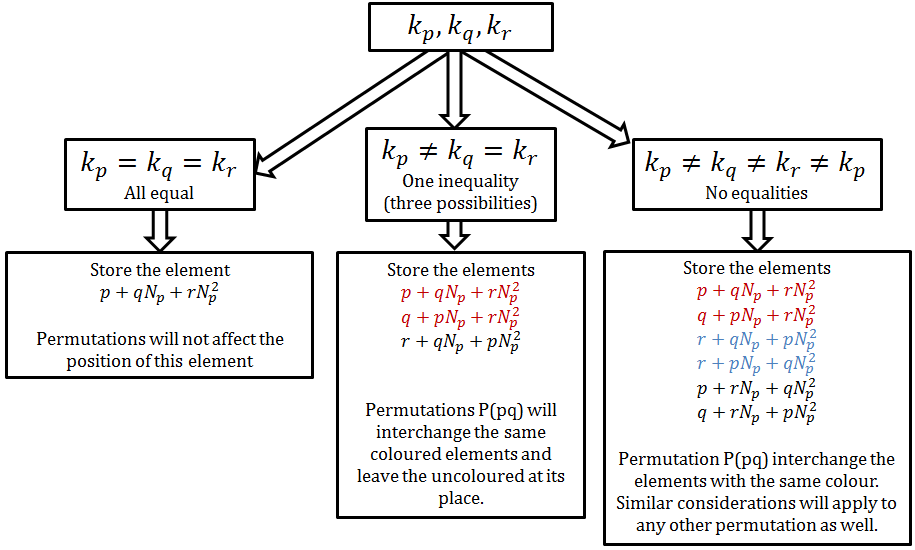
\includegraphics[width=0.8\textwidth]{permute_flow}
    \caption{Flowchart for the permutation and block identification algorithm.}
    \label{fig:permute_flow}
\end{figure}

\begin{figure}[p]
    \centering
    \includegraphics[width=0.8\textwidth]{BlockPermutations}
    \caption{Permuting a continuous image as a $t3$ amplitude stored as block matrices.}
    \label{fig:BlockPermutations}
\end{figure}

The equivalent command exists also for column ordering. 

\section{Element storage}

As opposed to the sparse implementation, we now only need to store rows and columns for the blocks in the interaction. All matrix elements are then calculated on the fly, since our interaction is not that computationally intensive.

In the case of the amplitudes, we also need to store the actual elements. In this case we must also store the full blocks. While the $t3$ elements are stored in a large, one-dimensional contiguous array of doubles, the different alignments are stored as blocks where each element corresponds to a position in the $t3$ element array. This setup is illustrated in Fig. \ref{fig2}. A closeup of the blocks is shown in Fig. \ref{fig:blocks_setup3}. 

The procedure of generating these blocks may be outlined as follows: To make sure each alignment refers to the same elements in the $t3$ element array, we begin by storing a unique unsigned integer (unsigned long long) for each nonzero index from the full tensor matrix in a array associated with the $t3$ elements. These elements may be be assigned values as

\begin{equation}
t^{abc}_{ijk} = a+ bN_p + cN_p^2 + iN_p^3 + jN_p^3 N_h+ kN_p^3 N_h^2.
\end{equation}

This number may unambiguously point us back to all the indices of the element in the full tensor matrix when needed.

When all nonzero elements are found in the channels needed for the diagram, we consolidate the elements stored in this array with the existing elements present in the tensor. If none are previously initialized, we may simply start assigning the indices from the $t3$ element array to the elements in the blocks starting with element 0. If elements are already present, we must update our blocks to point to the correct address in the element array. New elements may be added to the end of the element array.

Elements already present are found simply by identifying equal elements in the two unique unsigned integer arrays.

\begin{figure}[p]
    \centering
    \includegraphics[width=1\textwidth]{blocks_setup2}
    \caption{The relation between the contiguous array containing amplitudes and the partitioned blocks.}
    \label{fig2}
\end{figure}


\begin{figure}[p]
    \centering
    \includegraphics[width=0.8\textwidth]{vpppp_diagonal}
    \caption{Closeup of some block matrices in the pppp interaction.}
    \label{fig:vpppp_diagonal}
\end{figure}

\begin{figure}[p]
    \centering
    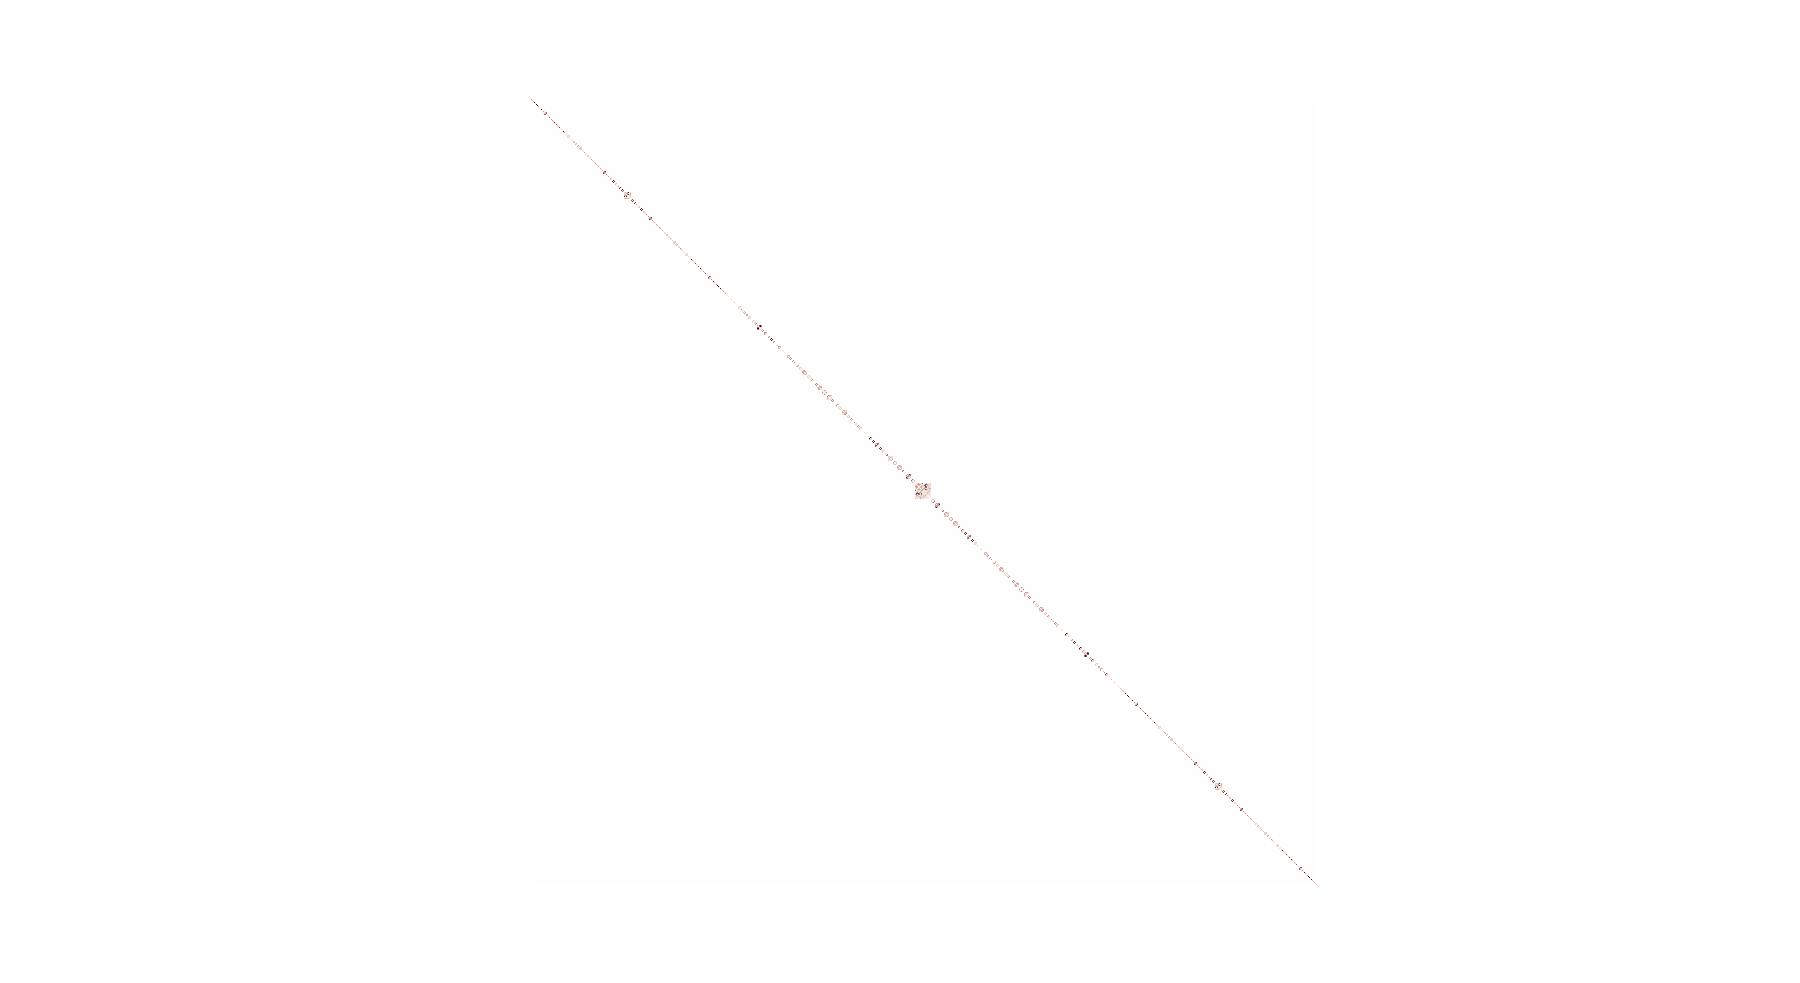
\includegraphics[width=0.8\textwidth]{vpppp_selection}
    \caption{All blocks for the pppp interaction for 66 basis states.}
    \label{fig:vpppp_selection}
\end{figure}

\begin{figure}[p]
    \centering
    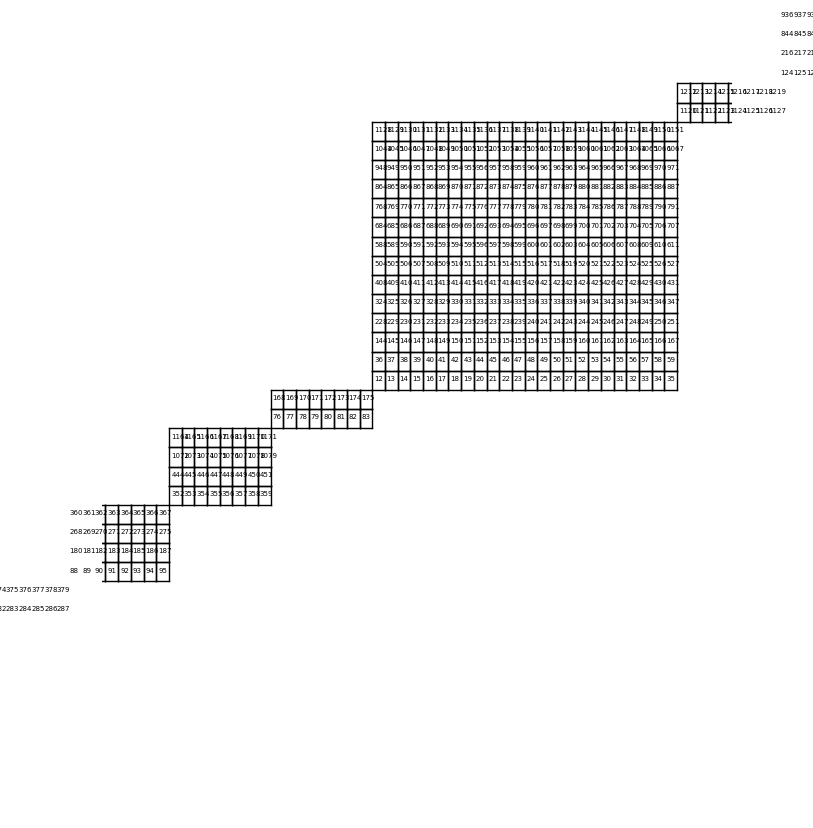
\includegraphics[width=0.8\textwidth]{bloks_setup3}
    \caption{Closeup of some block matrices in the amplitude.}
    \label{fig:blocks_setup3}
\end{figure}


\section{A sparse crossower scheme}

Upon mapping the aligned blocks needed for the various CCDT-1 diagrams, we find that the number of channels appearing in each diagram is lower than the number of unique configurations in the diagram's constituent tensors. This makes it possible to reduce memory usage, since we for any alignment need only store those blocks that appears in this intersection. 

All contributions to the $t3$ amplitude in the CCDT-1 method comes from contractions between the interaction and a linear $t2$ amplitude in diagrams $T_{1a}$ and $T_{1b}$. When adding in this contributions in the $t2$ equations through diagram $D_{10b}$ and $D_{10c}$, we will find that the alignment used for the $t3$ amplitude in $D_{10c}$ is actually the same as the one used to realign diagram $T_{1b}$. 

The only time we actually need the "naturally" aligned blocks from $t^{abc}_{ijk}$ is when we perform the permutations. 

Although the conservation arguments that define our blocks ensure that a given alignment corresponds to certain channels in the diagrams, they do not guarantee that the "naturally" aligned elements will belong to the same block. In fact, we will find that when we first set up the alignments needed before mapping the "natural" alignment, all the blocks in the "natural" alignment will have nonzero elements.

This means that we must map and perform permutations of \emph{all} the channels in the "natural" alignment. Such a process will consume a lot of memory and computing power to store and process a great deal of elements containing zeros. In the actual implementation, these difficulties are avoided by using a scheme inspired by parts of the sparse algorithm. 

We first map the three alignments needed for the four different diagrams. When all these elements are consolidated with the element array in the tensor, we map the "natural" alignment needed for permutations in a similar way as before. The only two differences will be that when we encounter elements not already present in the $t3$ amplitude, we let them vanish, and when we encounter values present in the $t3$ tensor we store them in an unsorted COO format together with the number of rows and columns of the matrix. It is then very easy to reconstruct the dense matrix when needed, and it reduces the memory consumption significantly.

Permutations are stored and performed exactly as described in the previous section.







